\chapter{Empirical Basis Functions for Max-stable Spatial Dependence}
\chaptermark{Empirical Basis Functions}
\label{appendix:c}

\section{Extreme value distributions} \label{eba:GEV}
The cumulative distribution function for the GEV is $F(y) = \exp\{-t(y)\}$ where
\begin{align} \label{ebeq:gevt}
  t(y) = \begin{cases}
      \left[1 + \xi \displaystyle \frac{y - \mu}{\sigma}\right]^{-1 / \xi}, \quad &\xi \neq 0 \\
      \\
      \exp\left\{- \displaystyle \frac{y - \mu}{\sigma}\right\}, &\xi = 0.
  \end{cases}
\end{align}
The probability density function for the GEV is given by $f(y) = \displaystyle \frac{1}{\sigma} t(x)^{\xi + 1} \exp\{-t(y)\}$ where $t(y)$ is defined in \eref{ebeq:gevt}.

\section{Grid approximation to PS density} \label{eba:gridapprox}
The PS($\alpha$) density can be challenging to use because it does not have a closed form.
From Section 2 of \citep{Stephenson2009}, the density can be expressed as
\begin{align}
  g_1(A) = \int_0^1 g_1(A, B) \dd B,
\end{align}
where
\begin{align}
  g_1(A, B) = \frac{\alpha}{1 - \alpha} \left( \frac{1}{A} \right)^{1 / 1 - \alpha} c(\pi B) \exp \left\{ -\left(\frac{1}{A}\right)^{\alpha / (1 - \alpha)} c(\pi B) \right\},
\end{align}
with
\begin{align}
  c(\psi) = \left[\frac{\sin(\alpha \psi)}{\sin(\psi)}\right]^{1 / (1 - \alpha)} \frac{\sin[(1 - \alpha) \psi]}{\sin(\alpha \psi)}.
\end{align}
\Citet{Stephenson2009} presents an auxiliary variable technique to deal with the integral in the density function, but we opt to numerically evaluate the integral because it is only one-dimensional.
To evaluate the integral, we use 50 evenly spaced quantiles of a Beta$(0.5, 0.5)$ distribution as the midpoints $B_1, \ldots, B_{50}$, and then use the midpoint rule to evaluate $\displaystyle \int_0^1 g_1(A, B) \dd B$.

\section{Standardized Gaussian kernel functions} \label{eba:gskfunctions}
\citet{Reich2012} use standardized Gaussian kernel functions as their spatial basis functions in the low-rank max-stable model.
Consider a set of $\bk_1, \ldots, \bk_L$ spatial knot locations in $\calD^2$, the region of interest.
Then
\begin{align}
  \hat{B}_{il} = \frac{\exp\left\{- \displaystyle\frac{||\bs_i - \bk_l||^2}{2 \rho^2} \right\}}{\displaystyle \sum_{j = 1}^L \exp\left\{- \frac{||\bs_i - \bk_j||^2}{2 \rho^2} \right\}}
\end{align}
where $|| \cdot ||$ is the Euclidean distance between a site and a knot location.

\section{Principal components} \label{eba:pca}
As a comparison to the EBFs, \fref{ebfig:fire-eigpanel} gives the first six principal components for the fire data, and \fref{ebfig:precip-eigpanel} gives the first six principal components for the precipitation data.
These figures show that the EBFs resemble the EOFs  for the uncersored precipitation data, but are quite different that the EOF from the censored fire data.
This is not surprising considering that the censoring results in only a small subset of data being used to estimate dependence.
\begin{figure}[htbp] % markdown/fire-analysis/basis-functions.R
  \centering
  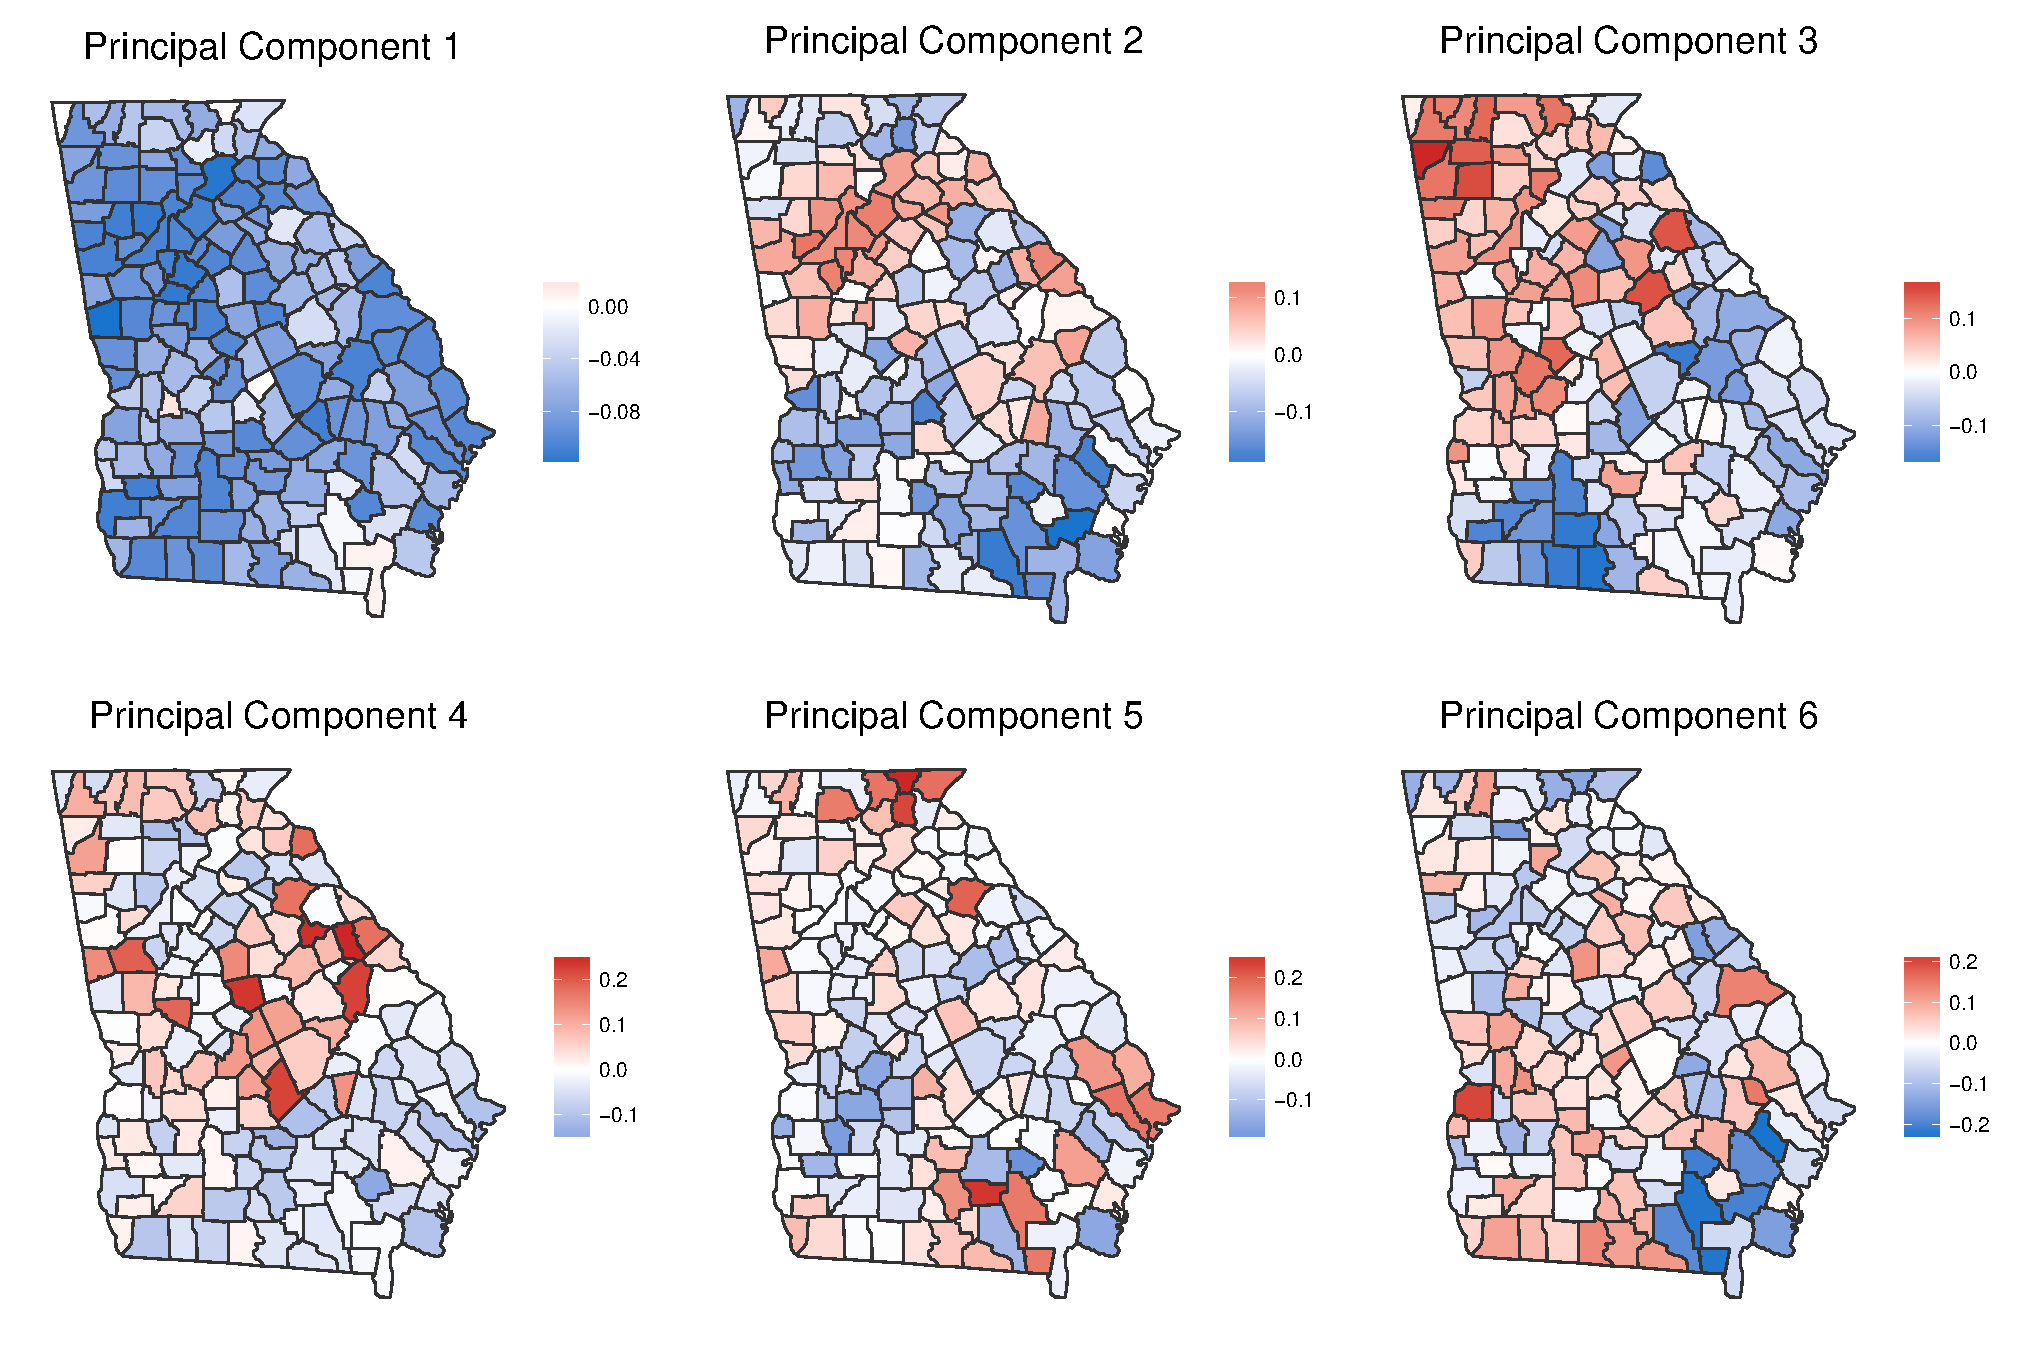
\includegraphics[width=\linewidth]{plots/fire-eig-panel.pdf}

  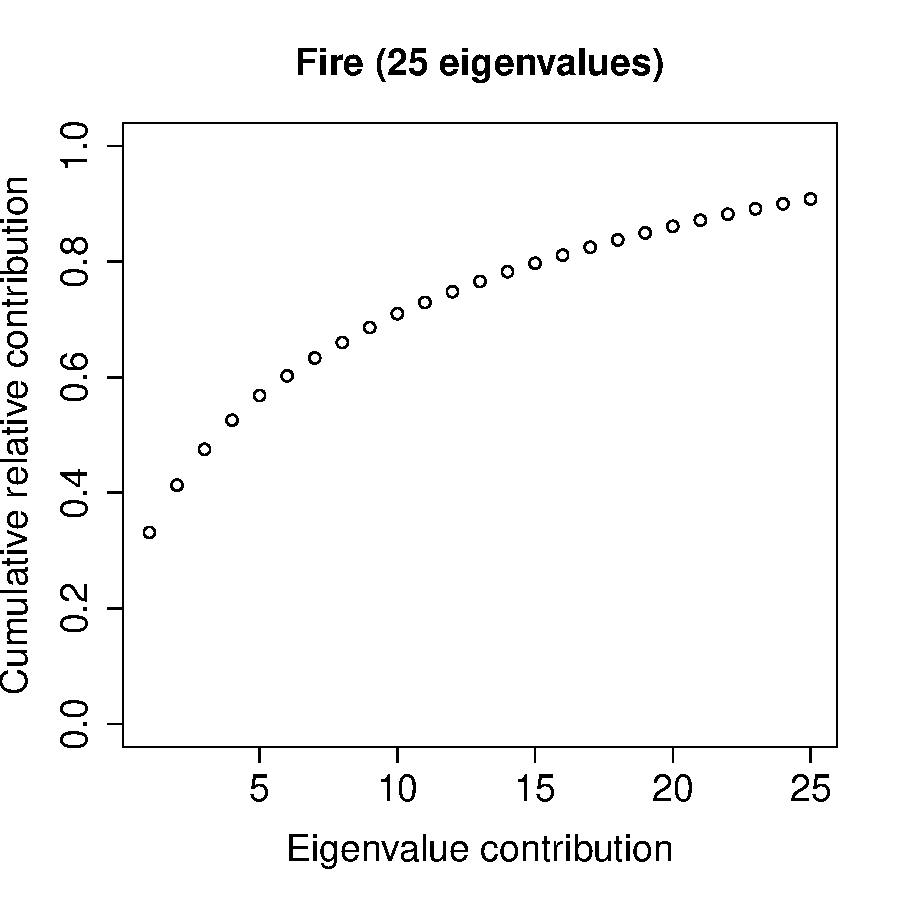
\includegraphics[width=0.35\linewidth]{plots/firelambda-25.pdf}
  \caption{First six principal components and the cumulative sum of the first 25 eigenvalues for the Georgia fire data.}
  \label{ebfig:fire-eigpanel}
\end{figure}

% \begin{figure}[htbp] % markdown/fire-analysis/basis-functions.R
%   \centering
%   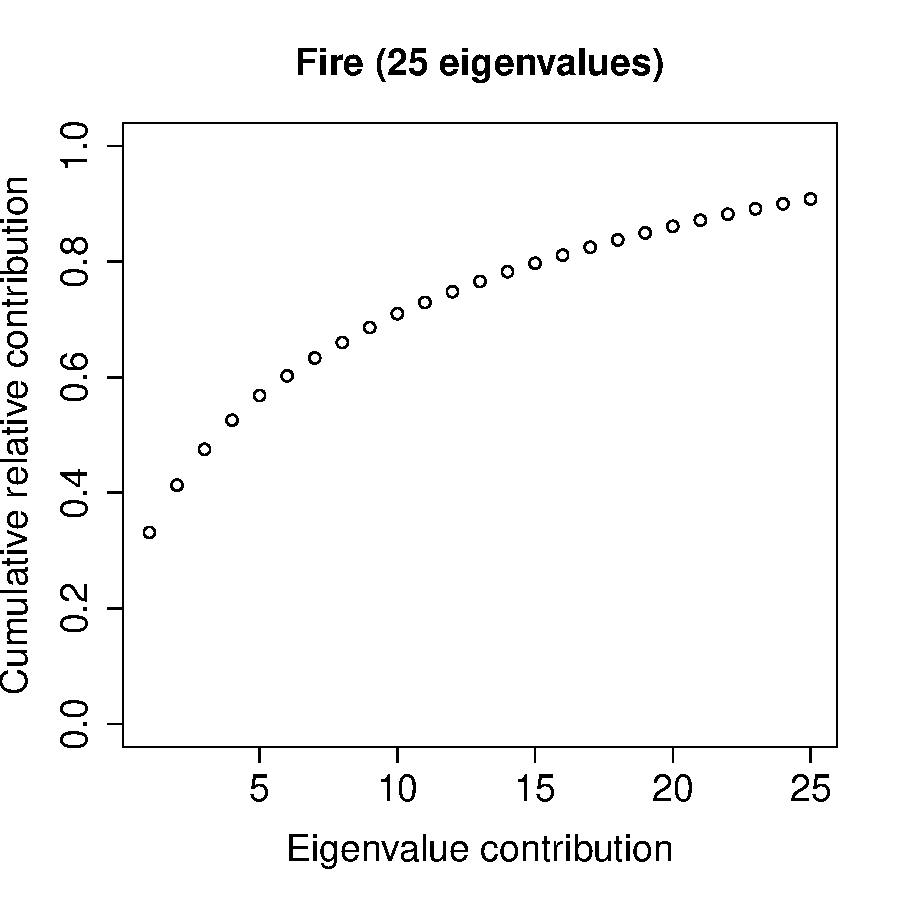
\includegraphics[width=0.5\linewidth]{plots/firelambda-25.pdf}
%   \caption{Cumulative sum of the first 25 eigenvalues.}
%   \label{ebfig:fire-eigpanel}
% \end{figure}

\begin{figure}[htbp]  % markdown/precipitation/cv-setup.R
  \centering
  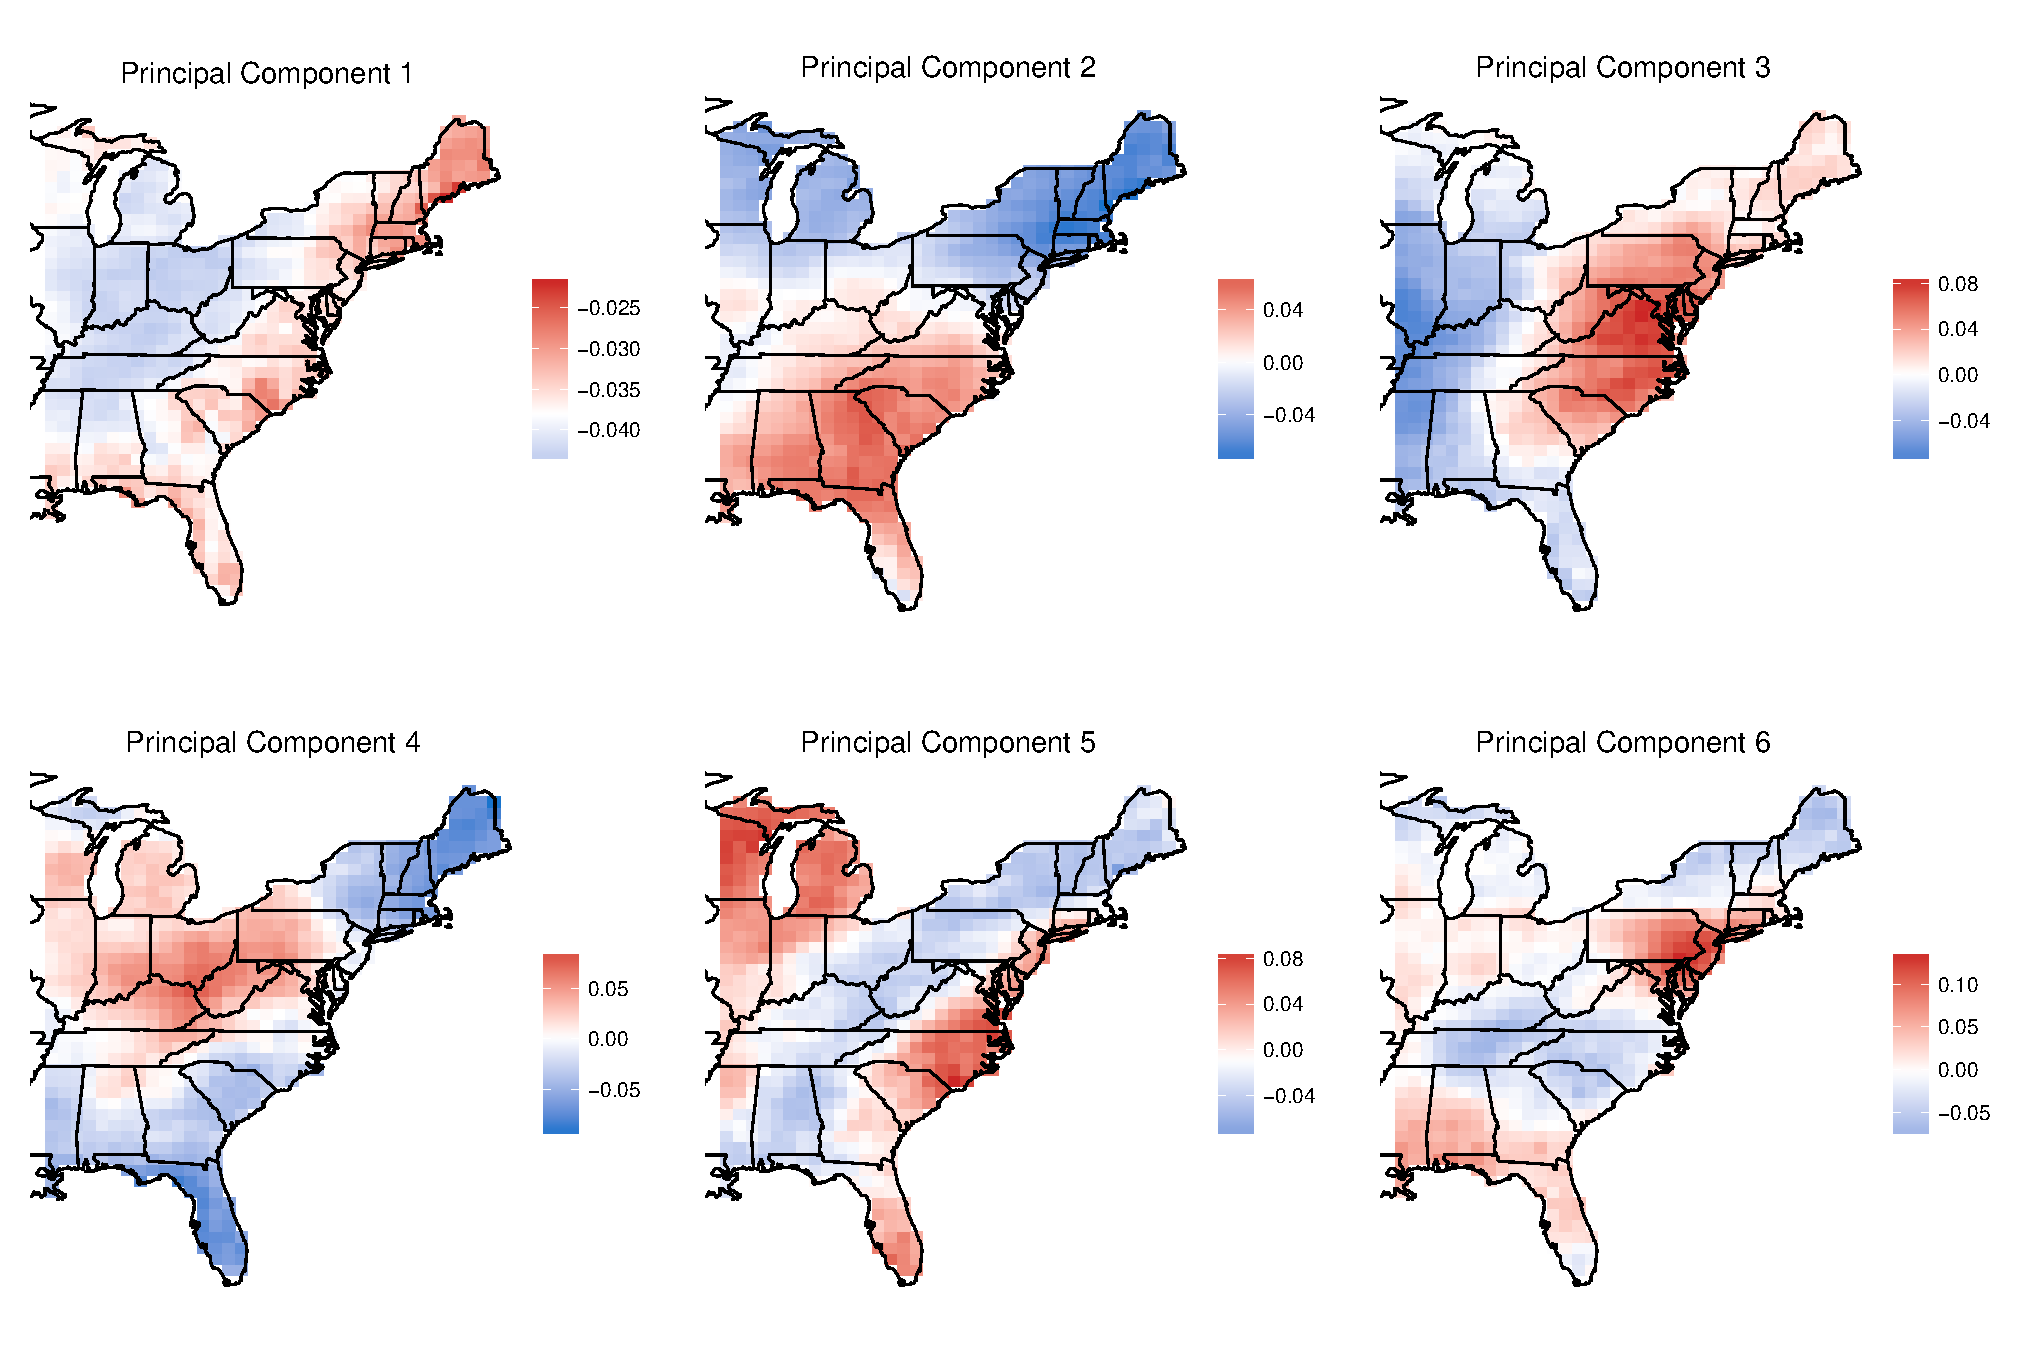
\includegraphics[width=\linewidth]{plots/precip-eig-panel.pdf}

  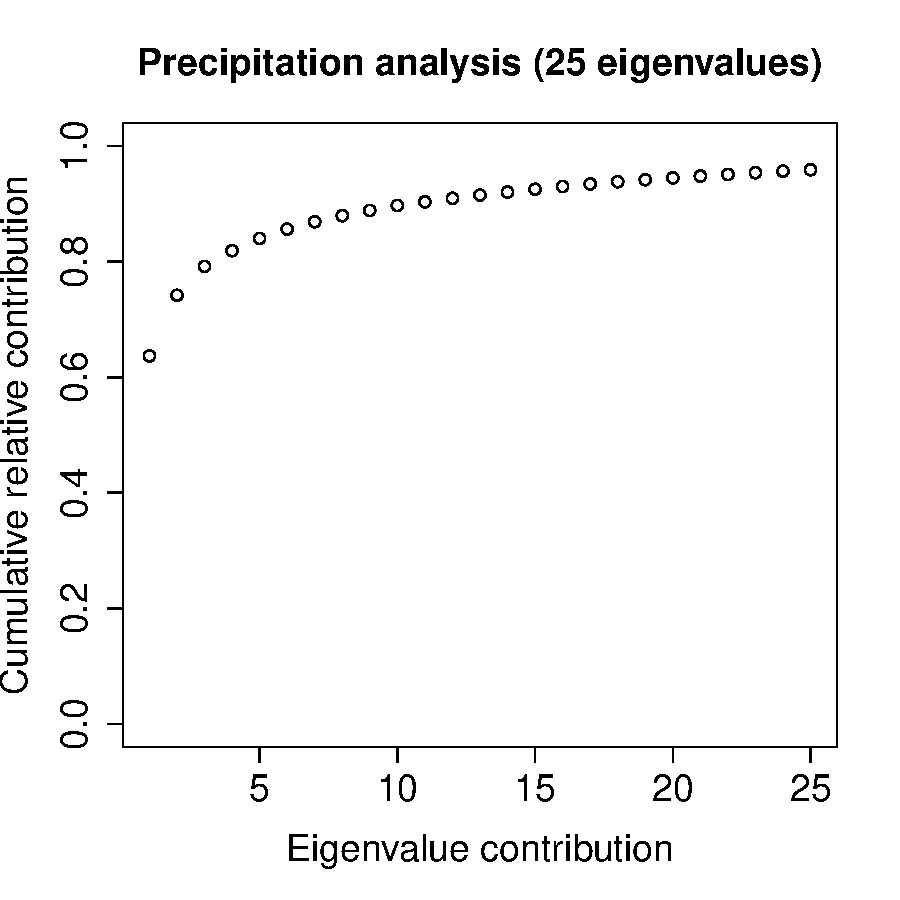
\includegraphics[width=0.35\linewidth]{plots/preciplambda-25.pdf}
  \caption{First six principal components and the cumulative sum of the first 25 eigenvalues for the precipitation data.}
  \label{ebfig:precip-eigpanel}
\end{figure}